\documentclass[12pt,a4paper]{report}
\usepackage{amsmath,amsthm,amssymb}
\usepackage[utf8]{inputenc}
\usepackage[russian]{babel}
\usepackage[T2A]{fontenc}

\usepackage{mathtext}
\usepackage{graphicx}

\usepackage{cmap}


\DeclareMathSizes{12}{14}{10}{8}

\usepackage[left=30mm, right=15mm, top=20mm, bottom=20mm]{geometry}
\usepackage{indentfirst}
\usepackage{setspace}
\usepackage{multirow,makecell,array}
\usepackage{cite} 
\usepackage{enumerate}
\hyphenpenalty=10000 

%\usepackage{float}
\usepackage{floatrow}
\usepackage{calc}

\makeatletter
\bibliographystyle{utf8gost705u}
\usepackage{titlesec}
\usepackage[usenames]{color}
\usepackage{colortbl}
\setcounter{secnumdepth}{5} 
\usepackage{tocloft} 

\renewcommand{\tiny}{\fontsize{7}{8.4pt}\selectfont}
\renewcommand{\scriptsize}{\fontsize{9}{11pt}\selectfont}
\renewcommand{\footnotesize}{\fontsize{11}{13.6pt}\selectfont}
\renewcommand{\small}{\fontsize{12}{14.5pt}\selectfont}
\renewcommand{\normalsize}{\fontsize{14}{18pt}\selectfont}
\renewcommand{\large}{\fontsize{17}{20pt}\selectfont}
\renewcommand{\Large}{\fontsize{20}{25pt}\selectfont}

\usepackage{hyperref}
\providecommand{\phantomsection}{}


\newcommand{\ket}[1]{\left|#1\right\rangle}
\newcommand{\bra}[1]{\left\langle #1\right|}

\newcommand{\NL}[2]{#1_{\mbox{\tiny #2}}}

\newcommand{\VSD}{\NL{V}{SD}}
\newcommand{\VG}{\NL{V}{G}}
\newcommand{\kBT}{k_{\mbox{\tiny B}}T}
\newcommand{\sgn}{\mbox{sgn}}

\newcommand{\Cis}[1]{C^{\mbox{\tiny о}}_{#1}}
\newcommand{\hCis}{\hat{C}^{\mbox{\tiny о}}}
\newcommand{\Cel}[1]{C^{\mbox{\tiny э}}_{#1}}
\newcommand{\hCel}{\hat{C}^{\mbox{\tiny э}}}
\newcommand{\Cisel}[1]{C^{\mbox{\tiny о-э}}_{#1}}
\newcommand{\hCisel}{\hat{C}^{\mbox{\tiny о-э}}}

\newcommand{\qis}{q^{\mbox{\tiny о}}}
\newcommand{\qel}{q^{\mbox{\tiny э}}}
\newcommand{\nis}{n^{\mbox{\tiny о}}}
\newcommand{\nel}{n^{\mbox{\tiny э}}}
\newcommand{\phiis}{\phi^{\mbox{\tiny о}}}
\newcommand{\phiel}{\phi^{\mbox{\tiny э}}}

\DeclareFloatSeparators{mysep}{\hspace{1cm}}%какая-то штука для картинок в ряд, вроде расстояние между плавающими объектами
\DeclareFloatSeparators{mysep2}{\hspace{2cm}}

\begin{document}

% настройка отступов
\setlength{\parindent}{1.25cm} 
% убираем висячие строки  и подобное безобразие
\sloppy   
% Запрещаем разрыв страницы после первой строки абзаца
\clubpenalty=10000		
% Запрещаем разрыв страницы перед последней строкой абзаца
\widowpenalty=10000		

% Полуторный интервал
\onehalfspacing  
%%%%%%%%%%%%%%%%%%%%%%%%%%%%%%%%%%%%%%%%%%%%%%%%%%%%%%%%
%                    Титульный лист                    %
%%%%%%%%%%%%%%%%%%%%%%%%%%%%%%%%%%%%%%%%%%%%%%%%%%%%%%%%
\thispagestyle{empty}
\begin{titlepage}
\begin{center}
ФЕДЕРАЛЬНОЕ ГОСУДАРСТВЕННОЕ БЮДЖЕТНОЕ ОБРАЗОВАТЕЛЬНОЕ
УЧРЕЖДЕНИЕ ВЫСШЕГО ОБРАЗОВАНИЯ \\
«МОСКОВСКИЙ ГОСУДАРСТВЕННЫЙ УНИВЕРСИТЕТ\\
имени М.В.ЛОМОНОСОВА»
\vspace{1cm}

ФИЗИЧЕСКИЙ ФАКУЛЬТЕТ\\
\vspace{1cm}
КАФЕДРА ФИЗИКИ ПОЛУПРОВОДНИКОВ И КРИОЭЛЕКТРОНИКИ\\

\vspace{1cm}
БАКАЛАВРСКАЯ РАБОТА \\
\vspace{1cm}

\textbf{<<ИССЛЕДОВАНИЕ ТРАНСПОРТНЫХ ХАРАКТЕРИСТИК ОДНОЭЛЕКТРОННОГО ОДНОАТОМНОГО ТРАНЗИСТОРА>>}


\end{center}


\begin{flushright}
\vspace{1cm}

Выполнил студент \\
416 группы:\\

Назаров Степан Сергеевич \\

\underline{\hspace{3cm}}\\

\vspace{1cm}

Научный руководитель:\\
доцент, к.ф.\--м.н. Шорохов В.В. \\
\underline{\hspace{3cm}}\\
 
\end{flushright}

\vspace{1cm}
\begin{flushleft}
Допущена к защите \\
Зав. кафедрой профессор О.В.Снигирев

\underline{\hspace{3cm}} \\
\end{flushleft}
\begin{center}
\vspace{1cm}
\small МОСКВА \\ \number\year\normalsize
\end{center}
\end{titlepage}



%%%%%%%%%%%%%%%%%%%%%%%%%%%%%%%%%%%%%%%%%%%%%%%%%%%%%%%%
%                      Оглавление                      %
%%%%%%%%%%%%%%%%%%%%%%%%%%%%%%%%%%%%%%%%%%%%%%%%%%%%%%%%
\setcounter{page}{2}
\tableofcontents

\chapter*{Введение}
\addcontentsline{toc}{chapter}{Введение}
%Работа первого одноэлектронного транзистора была продемонстрирована ещё в 1987 г.  \cite{Fulton_Dolan}. Основным принципом работы данного устройства является коррелированный во времени и пространстве транспорт электронов. Для 

Одноэлектронные устройства — это такие устройства, принцип работы которых основан на явлении коррелированного в пространстве и времени транспорта единичных электронов через зарядовые центры, представляющие собой обособленные металлические островки, соединённые с электродами и между собой туннельными переходами. Обязательным требованием к таким устройствам является достаточно низкое значение собственных и взаимных ёмкостей электродов и зарядовых островков. Это необходимо для того, чтобы изменение электростатической энергии системы за единичный акт туннелирования электрона было много больше энергии тепловых флуктуаций.

Первые работы, сообщающие о реализации устройств данного типа появились более 30 лет назад \cite{Fulton_Dolan, Amman, Likharev} и нашли применения в самых разных сферах:  термометрия\cite{Thermo}, память\cite{memory}, сенсоры\cite{sensor}.

Развитие технологических процессов в области изготовления полупроводниковых микросхем, привело к увеличению разрешающей способности, что позволяет уменьшить характерные размеры островков в устройствах. В наши дни на передовой находятся устройства с одиночными молекулами или атомами в роли зарядового центра \cite{SASET_EXP_OUR, SMSET}.

Нельзя не упомянуть резервуарные вычислительные нейросети, первые шаги к созданиям которых уже были проделаны в работе \cite{neuro}. Сами авторы считают, что кластер наночастиц золота можно рассматривать, как набор туннельно связанных одноатомных одноэлектронных транзисторов. 

Пока не существует технологического процесса, позволяющего в производственных масштабах изготавливать структуры из единичных атомов с допусками в единицы ангстрем. Уже были проведены теоретические работы по созданию обобщённых алгоритмов расчёта обычных одноэлектронных устройств \cite{Dobr}, где в роли зарядовых центров выступают металлические островки. Однако, с точки зрения практических применений (создание сенсоров, логических элементов) больший интерес проявляется к элементам из одиночных атомов и молекул. А значит, разработка универсальных методик расчёта для структур с дискретной энергетической структурой существенно расширит возможности на стадии проектирования подобного рода устройств.



\section*{Цель работы}

Целью данной бакалаврской работы является создание универсального алгоритма расчёта структур с атомной функциональной структурой, анализ и моделирование систем с такими структурами в роли ключевых элементов и применение данного алгоритма для объяснения наблюдаемых в эксперименте характеристик одноатомных одноэлектронных устройств.


\chapter{Методики расчёта одноэлектронного транспорта}
Одноэлектронный транзистор состоит из маленького металлического островка субмикронных размеров, двух электродов исток-сток соединённых с островком туннельно и электрода затвор, изолированного от острова. Схематично это устройство изображено на рис. \ref{fig:SET}. На рисунке так же указаны параметры: $C_S, C_D, C_G$ — ёмкости соответствующих переходов; $R_S, R_D$ — соответствующие туннельные сопротивления.

\begin{figure}
	\center{\includegraphics[scale=0.3]{SET.jpg}}
	\caption{Одноэлектронный транзистор}
	\label{fig:SET}
\end{figure}

Работа такого транзистора возможна только при выполнении двух очень важных условий:
\begin{equation}\label{c1}
\frac{e^2}{2C} >> kT
\end{equation}
\begin{equation}\label{c2}
R_S >> R_Q, R_D >> R_Q,  R_Q = h/e^2
\end{equation}
Первое условие о преобладании изменения электростатической энергии системы за единый акт туннелирования над энергией тепловых флуктуаций. В формуле (\ref{c1}) $C = C_S + C_D + C_G$ — суммарная ёмкость системы. Условие (\ref{c2}) говорит о том, что мы так же пренебрегаем ещё и квантовыми флуктуациями электронов. $R_Q = 25.8$ кОм — так называемое квантовое сопротивление.

В основополагающей работе \cite{Fulton_Dolan} размер острова был порядка $1\mu m$. В работе 2002 г. \cite{SASET1} Зазор между туннельными электродами был уже порядка 1-2 $nm$. Стоит отметить что для современных одноатомных транзисторов величина зазора не стала на порядок меньше, а находится на том же уровне, или чуть меньше 1 $nm$. Очевидно, что ёмкость системы пропорциональна её энергетическим размерам: $C \sim r$. Уменьшение размеров устройств позволило отодвинуть границу рабочей температуры, фигурирующей в (\ref{c1}).

Возможность создания столь малых структур позволила в роли островков использовать отдельные примесные атомы \cite{SASET_EXP_OUR, SMSET}. Однако, электрон в атоме может пребывать только в строго определённых дискретных энергетических состояниях, в то время как в распределённом металлическом островке распределение энергетических состояний электрона практически непрерывно.

Учитывая последнее обстоятельство, становится ясно, что классическая (ортодоксальная)\cite{Likharev} теория одноэлектроники при рассмотрении одноатомных одноэлектронных транзисторов  неприменима. Соответственно, для рассчёта характеристик таких устройств необходимо составление отдельной физической модели явления и её расчёт.
\section{Модель Хаббарда}

Модель Хаббарда — приближение, используемое в физике твёрдого тела для описания перехода между проводящим и диэлектрическим состояниями \cite{Hubbard}. Гамильтониан системы в этой модели даётся следующим соотношением:
\begin{equation}
\hat{H} = -t \sum\limits_{<i, j>, \sigma}(\hat{a}_{i, \sigma}^{\dagger}\hat{a}_{i + 1, \sigma} + \hat{a}_{i+1, \sigma}^{\dagger}\hat{a}_{i, \sigma}) + U \sum\limits_{i}\hat{n}_{i \uparrow} \hat{n}_{i \downarrow}
\end{equation}
где $\hat{n}_{i \sigma} = \hat{a}_{i, \sigma}^{\dagger} \hat{a}_{i, \sigma}$  — оператор спин-плотности для электрона со спином $\sigma$ на i-ом уровне. $\hat{a}_{i, \sigma}^{\dagger}$ и $ \hat{a}_{i, \sigma}$ представляют собой операторы рождения и уничтожения фермионов, используемые в формализме вторичного квантования.$<i, j>$ означает ближайшие узлы в решётке. Первое слагаемое в данном гамильтониане является перескоковым интегралом <<t>>, отвечающим за кинетическую энергию электронов. Второе — внутриузельное отталкивание <<U>>, соответствующее потенциальной энергии кулоновского отталкивания электронов. Без второго слагаемого гамильтониан Хаббарда становится гамильтонианом сильной связи из стандартной зонной теории. Часто $\hat{a}_{i+1, \sigma}^{\dagger}\hat{a}_{i, \sigma}$ обозначают как $h.c.$ — эрмитово сопряжённое слагаемое.

\section{t-J модель}
t-J модель\cite{tJ} была выведена в 1977 году из модели Хаббарда. Данная модель описывает сильно коррелированные системы электронов и используется для расчёта уровней в высокотемпературных сверхпроводниках в допированных антиферромагнетиках. Гамильтониан в этом приближении:
\begin{equation}
\hat{H} = -t \sum\limits_{<i, j>, \sigma}(\hat{a}_{i, \sigma}^{\dagger}\hat{a}_{i + 1, \sigma} + h.c.) + \frac{1}{2}J \sum\limits_{<i, j>}(\vec{S_i} \vec{S_j} - \frac{n_i n_j}{4})
\end{equation}
Здесь $J = \frac{4 t^2}{U}$ — константа связи, $\vec{S_i}, \vec{S_j}$ — спины в состояниях  i, j. $n_i = \sum\limits_{\sigma} \hat{a}_{i, \sigma}^{\dagger} \hat{a}_{i, \sigma}$ — количество частиц на уровне i.

После того, как выписан Гамильтониан системы зачастую применяется формализм функций Грина\cite{Masl}, на основе которых рассчитываются матричные элементы туннельных операторов и составляются кинетические уравнения для расчёта туннельного тока в системе.

\section{Полуфеноменологическая модель}

В данной работе мы пойдём другим путём и уйдём от формализма квантовой механики в сторону квазиклассического описания, с прицелом на то, что такой подход позволит повысить производительность расчётов, позволит обсчитывать транспортные характеристики систем с большим количеством уровней, зарядовых центров и зарядовых состояний.

Первым делом запишем выражение для энергии системы в некотором её зарядовом состоянии:
\begin{equation}\label{phen}
E = \sum\limits_{<i>}E_i n_i + \frac{1}{2} \sum\limits_{i \neq j} U_{ij} n_i n_j
\end{equation}
$E_i$ здесь представляют собой энергии уровней в атоме для электронов, а $U_{ij}$ — константы взаимодействия электронов на разных энергетических уровнях. Заметим, что энергия системы записанная таким образом очень похожа на то, что мы имели в моделях, описанных выше.

Если оценка $E_i$ не вызывает трудностей(ведь это суть есть энергетический спектр атома, значения которого можно взять из экспериментальных данных), то вопрос оценки $U_{ij}$ более интересен. Во-первых, стоит учесть кулоновское взаимодействие:
\begin{equation}
U_{ij}^{(1)} = \int \int \frac{e^2 |\varphi_i(\vec{r})|^2 |\varphi_j(\vec{r})|^2 dV_i dV_j}{r_{ij}}
\end{equation}
$\varphi_i(\vec{r})$ — одночастичная волновая функция электрона, во-вторых, корреляционную поправку на энергию взаимодействия:
\begin{equation}
U_{ij}^{(2)} = \int \int \frac{(1 - g(\vec{r_{ij}})) \rho_i \rho_j dV_i dV_j}{r_{ij}}
\end{equation}
и, в третьих, поправку на обменное взаимодействие:
\begin{equation}
U_{ij}^{(3)} = \int \int \frac{\varphi_i(\vec(r_i)) \varphi_j(\vec(r_j)) \varphi_i^{*}(\vec(r_j))\varphi_j^*(\vec(r_i)) dV_i dV_j}{r_{ij}}
\end{equation}

Однако в данной работе мы будем использовать только вклад от кулоновского отталкивания. На то есть две причины:
\begin{itemize}
\item Данная работа больше сфокусирована на том, как из заявленных величин в выражении для полной энергии получить транспортные характеристики транзистора
\item Указанные константы всегда можно получить из программного пакета квантовой химии, например NWChem, вставить в написанную в ходе данной работы программу и рассчитать транспортные характеристики для транзистора, на основе интересующего нас конкретного атома или молекулы
\end{itemize}


Следует уточнить, что данная модель применима при слабой связи зарядовых центров с электродами и друг с другом (в случае многоостровковых систем), т.е. когда электронный транспорт в системе является преимущественно одноэлектронным. А это, как уже было упомянуто при выполнении условий (\ref{c1}), (\ref{c2}). Причём второе условие становится особенно важным в нашем рассмотрении, ведь оно говорит о том, что в расматриваемом случае одночастичные волновые функции электронов $\varphi_i(\vec{r})$ слабо перекрываются, что позволяет оперировать не самими волновыми функциями, а их эффективными радиусами локализации $r_{eff}$. А с помощью последних можно в свою дать оценки характерных энергетических величин кулоновского взаимодействия.

К слову об этих величинах. Константы взаимодействия из формулы \ref{phen} всегда можно переписать в следующем виде:
\begin{equation}
E_i = \frac{e^2}{2 C_{ii}}, U_{ij} = \frac{e^2}{2 C_{ij}}
\end{equation}

Очевидно, что говорить о настоящих электростатических ёмкостях при работе со структурами атомного масштаба не приходится. Величины $C_{ij}$ в формулах выше это не ёмкости в привычном их понимании. Это переписанные в удобном, узнаваемом виде энергетические константы, которые будет удобно оценивать с помощью $r_{eff}$. 

Ещё раз обратимся к условию (\ref{c2}). Записывая его в виде
\begin{equation}
\tau = |M_T|^2 = \frac{R_Q}{R_T D_1 D_2} << 1
\end{equation}
где $\tau$ — прозрачность туннельного барьера, $R_T$ — его сопротивление, $D_1, D_2$ — плотности электронных состояний на границах электродов, получаем требование на величину прозрачности барьера для применимости модели. И именно такие величины $\tau \approx 10^{-2} - 10^{-3}$ наблюдаются в эксперименте \cite{SASET_EXP_OUR, patriot}, а применение описываемой модели к расчёту транспорта в одноэлектронных системах в указанном диапазоне прозрачностей барьеров дало хорошее согласие с экспериментальными данными \textbf{*ссылка на работу с Ярославом*}.

На этом остановим идейное описание метода моделирования транспорта в системе и перейдём к конкретным оценкам.

\chapter{Расчёт полуфеноменологической модели}

Необходимо смоделировать работу  одноатомного одноэлектронного транзистора. Типичное его устройство представлено на рис.\ref{fig:SASET}. Этот транзистор исследовался в работе \cite{patriot}. Кремниевые электроды на подложке из оксида кремния. Между электродами находится примесный атом мышьяка. 
\begin{figure}[h]
	\center{\includegraphics[scale=0.3]{patriot.png}}
	\caption{Одноатомный одноэлектронный транзистор}
	\label{fig:SASET}
\end{figure}
Электроды представим как три относительно больших проводящих сферы. Здесь мы сразу же вспомним про уже введённые величины $C_{ij}$. Понятно, что размеры электродов колосально превышают линейный размер ключевого элемента(атома). И в перовм приближении неважно будет ли у электрода сферическая форма или же коническая. Наибольший вклад в $C_{ij}$, будут вносить его линейные размеры. К примеру, с удовлетворительной точностью можно считать $C_{ii} \approx R_i$ . $R_i$ — радиус сферы.

Примесный атом отождествим с двумя концентрическими проводящими сферами. Две последних отвечают за представление электронных оболочек атома. Тут мы воспользуемся требованием (\ref{c2}) к слабому перекрытию одночастичных волновых функций и будем считать что ВФ локализованы на расстояниях $r_i$ от центра атома в интервале расстояний намного меньшим, чем соответствующее $r_i$. Все геометрические размеры представлены на рис. \ref{fig:SASET model}.
\begin{figure}[h]
	\center{\includegraphics[scale=0.35]{SASET model}}
	\caption{Модель одноатомного одноэлектронного транзистора}
	\label{fig:SASET model}
\end{figure}

Каждая сфера из набора концентрических будет соответствовать отдельной оболочке и отдельному энергетическому уровню. Для наглядности и простоты вычислений пока ограничимся двумя. Мы так же пока не принимаем во внимание различие в формах атомных орбиталей в зависимости от их типа($s,p,d,f$). 

Так-же будем считать, что электроны могут туннелировать только со сфер Исток, Сток на сферы атома и в обратную сторону. Т.е. туннельного тока на Затвор нет.

Исток, Сток и Затвор поддерживаем при постоянном напряжении, то есть подаём на указанные сферы потенциалы $\varphi_s, \varphi_d, \varphi_g$ соответственно.

Нам так же потребуются значения энергии Ферми $\varepsilon_F$ для электродов и значения энергетического спектра атома $\mu_1, \mu_2$. Эти переменные будут давать прямой вклад в величины $E_i$, фигурирующие в (\ref{phen}). 

Оканчивая постановку задачи, необходимо найти значение силы тока электронов с Истока на Сток, при заданных потенциалах на электродах $\varphi_s, \varphi_d, \varphi_g$. А для получения диаграмм стабильности, найти ток в каждой точке некоторого диапазона изменения потенциалов.

\section{Изменение свободной энергии системы}
Начнём с расчёта изменения свободной энергии системы. При наличии 5 тел в системе становится удобен матричный подход к описанию зарядов и потенциалов, т.к. количество уравнений для расчёта будет расти как минимум пропорционально количеству тел.

Введём векторы зарядов и векторы потенциалов на рассматриваемых телах.
\begin{equation}
\vec{q} =  \left(
  \begin{array}{c}
    q_s\\
    q_d\\
    q_g\\
    q_1\\
    q_2\\
  \end{array}
  \right) = \left(
  \begin{array}{c}
  \vec{q_e}\\
  \vec{q_d}\\
  \end{array}
  \right)
  , 
  \vec{\varphi} = \left(
  \begin{array}{c}
  \varphi_s\\
  \varphi_d\\
  \varphi_g\\
  \varphi_1\\
  \varphi_2\\
  \end{array}
  \right) = \left(
  \begin{array}{c}
  \vec{\varphi_e}\\
  \vec{\varphi_d}\\
  \end{array}
  \right)
\end{equation}

Изменение энергии мы будем рассматривать за один акт туннелирования. Введём в рассмотрение начальные $\vec{\varphi}_{\mbox{i}}, \vec{q}_{\mbox{i}}$ и конечные $\vec{\varphi}_{\mbox{f}}, \vec{q}_{\mbox{f}}$ значения этих векторов. $\vec{q_e}, \vec{\varphi_e}$ — электродные компоненты векторов (от англ. electrode), так же являющиеся векторами, а $\vec{q_d}, \vec{\varphi_d}$ — атомные их компоненты (от англ. dopant). Для наглядности:
\begin{equation}
\vec{q_e} = \left(
\begin{array}{c}
q_s\\
q_d\\
q_g\\
\end{array}
\right),
\vec{\varphi_d} = \left(
\begin{array}{c}
\varphi_1\\
\varphi_2\\
\end{array}
\right)
\end{equation}

Изменение электростатической энергии запишем в виде
\begin{equation}
  dU = 
  \frac{\vec{\varphi_{f}^T}\vec{q}_{f}-\vec{\varphi_{i}^T}\vec{q}_{i}}{2}=
  \frac{(\vec{\varphi_{i}^T}+\vec{d\varphi^T})
  (\vec{q}_{i}+d\vec{q})
  -\vec{\varphi_{i}^T}\vec{q}_{i}}{2}
\end{equation}
Здесь $\vec{\varphi_{f}^T}$ — по сути строка, получающаяся транспонированием вектора. Заметим, поскольку электроды поддерживаются при постоянном потенциале, то 
вектор изменения потенциалов всех элементов 
\begin{equation}
  d\vec{\varphi}=
  \vec{\varphi}_{\mbox{f}}-\vec{\varphi}_{\mbox{i}}=
  \left(
  \begin{array}{c}
   \vec 0_e\\
   d\vec \varphi_d
  \end{array}
  \right)
\end{equation}
Вектор изменения зарядов всех элементов 
\begin{equation}
  d\vec{q}=
  \vec{q}_{\mbox{f}}-\vec{q}_{\mbox{i}}=
  \left(
  \begin{array}{c}
   d\vec q_{ind}+d\vec q_{tun}\\
   d\vec q_d
  \end{array}
  \right)=
  \left(
  \begin{array}{c}
   d\vec q_{ind}+ed\vec n_{tun}\\
   ed\vec n_d
  \end{array}
  \right),
\end{equation}
где $d\vec q_{ind}$ — вектор изменения индуцированных на электродах зарядах, $d\vec{n_{tun}}$ — вектор изменения заряда электродов вследствие туннелирования, $d\vec{n_d}$ — вектор изменения количества электронов на атомных уровнях.
Выражение для изменения свободной энергии можно переписать в следующем 
виде с учетом неизменности электрических потенциалов электродов
\begin{equation}
  dU = \frac{\vec{\varphi}^T_{\mbox{i}}d\vec{q}+
  \vec{q}^T_{\mbox{i}}d\vec{\varphi}+
  d\vec{q}^Td\vec{\varphi}}{2}=
  \frac{(\vec{q}^T_d+d\vec{q}^T_d)d\vec{\varphi}_d+
  \vec{\varphi}_d^Td\vec{q}_d+
  \vec{\varphi}_e^Td\vec{q}_{ind}}{2}
\end{equation}
Для нахождения $d\vec q_{ind}$, $\vec{\varphi}_d$ и 
$d\vec{\varphi}_d$ запишем систему уравнений
\begin{equation}\label{eq3}
  \left(
  \begin{array}{c}
   \vec q_{ind}\\
   \vec q_d
  \end{array}
  \right)=
  \left(
  \begin{array}{cc}
   \hat C_{ee} & \hat C_{ed}\\
   \hat C_{de} & \hat C_{dd}
  \end{array}
  \right)
  \left(
  \begin{array}{c}
   \vec \varphi_e\\
   \vec \varphi_d
  \end{array}
  \right)
\end{equation}
Более подробно о матрице, фигурирующей в последнем уравнении, поговорим в следующем параграфе. Пока достаточно считать, что между зарядами и потенциалами на телах существует линейная связь, что как раз и было продемонстрировано в работе \textbf{*Ссылка на работу с Ярославом*}. Отсюда получаем
\begin{equation}
  \begin{array}{l}
   \vec \varphi_d=\hat C^{-1}_{dd}
   (\vec{q}_d-\hat C_{de}\vec \varphi_e)\\
   \vec q_{ind}=(\hat C_{ee}-\hat C_{ed}\hat C^{-1}_{dd}\hat C_{de})\varphi_e+
   \hat C_{ed}\hat C^{-1}_{dd}\vec q_d.
  \end{array}
\end{equation}
На основе этих уравнений для $d\vec q_{ind}$ и 
$d\vec{\varphi}_d$ получаем:
\begin{equation}
  \begin{array}{l}
   d\vec \varphi_d=\hat C^{-1}_{dd}d\vec{q}_d\\
   d\vec q_{ind}=
   \hat C_{ed}\hat C^{-1}_{dd}d\vec q_d.
  \end{array}
\end{equation}
Получаем для изменения электростатической энергии
\begin{equation}
  dU = 
  \frac{(\vec{q}^T_d+d\vec{q}^T_d)\hat C^{-1}_{dd}d\vec{q}_d+
  (\vec{q}_d^T-\vec \varphi_e^T\hat C_{ed})\hat C^{-1}_{dd}d\vec{q}_d+
  \vec{\varphi}_e^T\hat C_{ed}\hat C^{-1}_{dd}d\vec q_d}{2}
\end{equation}
Окончательно изменения электростатической энергии:
\begin{equation}
  dU = \vec{q}^T_d\hat C^{-1}_{dd}d\vec{q}_d+
  \frac{d\vec{q}^T_d\hat C^{-1}_{dd}d\vec{q}_d}{2}=
  e^2\vec{n}^T_d\hat C^{-1}_{dd}d\vec{n}_d+
  \frac{e^2}{2}d\vec{n}^T_d\hat C^{-1}_{dd}d\vec{n}_d
\end{equation}
Изменение свободной энергии системы включает в себя работу источников
\begin{equation}\label{eq1}
 dF=dU + U=e^2\vec{n}^T_d\hat C^{-1}_{dd}d\vec{n}_d+
  \frac{e^2}{2}d\vec{n}^T_d\hat C^{-1}_{dd}d\vec{n}_d+
  e\vec \varphi_e^T(\hat C_{ed}\hat C^{-1}_{dd}d\vec{n}_d+d\vec{n}_{tun})
\end{equation}
\section{Матрица констант взаимодействия}
Для вычисления изменения свободной энергии требуется рассчитать матрицу , фигурирующую в (\ref{eq3}). Именно в этом месте стоит заметить, что выбранное нами обозначение для констант взаимодействия $C_{ij}$ не случайно, ведь в рамках линейной связи потенциалов и зарядов на телах в системе коэффициенты $C_{ij}$ действительно напоминают собственные и взаимные ёмкости тел в системе. Сделав данную оговорку далее будем называть коэффициенты $C_{ij}$ ёмкостями для краткости.%По сути само уравнение (\ref{eq3}) можно считать определением матрицы ёмкостей данной системы — элементы матрицы ёмкости есть коэффициенты в линейной комбинации потенциалов для выражения зарядов на объектах в системе.

Рассмотрим процедуру расчёта данной матрицы в нашей модели. Расчёту взаимных коэффициентов концентрических сфер мы посвятим следующий параграф, а пока остановимся на всех остальных элементах.
Для наглядности выпишем нашу матрицу в полном виде
\begin{equation}
\hat C = \begin{pmatrix}
C_{ss}& C_{sd}& C_{sg}& C_{s1}& C_{s2}\\
C_{ds}& C_{dd}& C_{dg}& C_{d1}& C_{d2}\\
C_{gs}& C_{gd}& C_{gg}& C_{g1}& C_{g2}\\
C_{1s}& C_{1d}& C_{1g}& C_{11}& C_{12}\\
C_{2s}& C_{2d}& C_{2g}& C_{21}& C_{22}\\
\end{pmatrix}
\end{equation}
Поясним: здесь $C_{ss}$ — собственная ёмкость истока, $C_{dd}$ — стока, $C_{gg}$ — затвора, $C_{11}$ — собственная ёмкость сферы первого энергетического уровня, $C_{22}$ — второго. К примеру,$C_{sd}$ — взаимная ёмкость стока и стока и т.д. Элементы $C_{11}, C_{12}, C_{21}, C_{22}$ оставляем на потом, а с остальными разберёмся уже сейчас. Вычислять их будем по отдельности: Первая группа будет состоять из элементов собственных и взаимных ёмкостей электродов (их всего 9, например $C_{gg}, C_{ds}$) а так же ещё шести элементов взаимной ёмкости первой сферы и электродов (это элементы вида $C_{s1}, C_{d1}, C_{1g}$ и т.д.). Вторая группа будет состоять из тех же девяти коэффициентов, относящихся к электродам, и ещё шести, связанных со второй сферой (вида $C_{s2}, C_{2g}$ и т.д.)

Разделив матрицу на 2 таких группы, мы можем рассчитать матрицу ёмкостей для двух систем четырёх непересекающихся и не лежащих внутри друг друга сфер. Сделать это можно с помощью метода изображений. Данный метод был детально описан в \cite{Landau}. Поместив пробный заряд на одну из сфер, будем последовательно строить заряды-изображения в других сферах до тех пор, пока поправка на величину заряда-изображения в $i$-ой итерации не станет меньше выбранного $\varepsilon$.

Раз мы уже затронули методы математической физики то не лишним будет сказать, что используя метод изображений, мы тем самым решаем задачу Дирихле для оператора Лапласа на плоскости \cite{MMF}. Аппроксимация электродов и атомных орбиталей с помощью сфер была выбрана как раз для того, чтобы не усложнять расчёты решением этой задачи в трёхмерном пространстве где тела бы представляли собой более сложные геометрические объекты. Тогда бы нам пришлось вводить координатную сетку в пространстве и решать задачу с помощью метода конечных разностей. Кратко говоря, учёт действительной геометрии системы является одним из способов значительного повышения точности расчётов.
\section{Потенциалы и заряды системы концентрических проводящих сфер}

Пусть имеется система проводящих концентрических сфер с радиусами 
$r_1<r_2<\dots<r_N$ и зарядами $q_i$. Тогда потенциал внешней сферы по теореме 
Остроградского-Гаусса определяется как
\begin{equation}
  \varphi_N=\frac{\sum\limits_{i=1}^Nq_i}{r_N}\,.
\end{equation}

Потенциал $N-1$ сферы определяется как
\begin{equation}
  \varphi_N=\frac{\sum\limits_{i=1}^{N-1}q_i}{r_{N-1}}+\phi_{N-1}\,,
\end{equation}
где константа $\phi_{N-1}$ определяется из условия
\begin{equation}
 \frac{\sum\limits_{i=1}^{N-1}q_i}{r_{N}}+\phi_{N-1}=
 \frac{\sum\limits_{i=1}^Nq_i}{r_N},\;
  \phi_{N-1}=\frac{q_N}{r_N}
\end{equation}

Таким образом, потенциалы и заряды на $N$ концентрических сферах определены 
равенством:
\begin{equation}
  \left(
  \begin{array}{c}
    \vec \varphi_1\\
    \vdots\\
    \vec \varphi_N
  \end{array}
  \right)=
  \left(
  \begin{array}{ccccccc}
1/r_1 & 1/r_2 & 1/r_3 & \ldots & 1/r_{N-2} & 1/r_{N-1} & 1/r_N\\
1/r_2 & 1/r_2 & 1/r_3 & \ldots & 1/r_{N-2} & 1/r_{N-1} & 1/r_N\\
1/r_3 & 1/r_3 & 1/r_3 & \ldots & 1/r_{N-2} & 1/r_{N-1} & 1/r_N\\
\vdots & \vdots & \vdots & \ldots & \vdots & \vdots & \vdots\\
1/r_{N-2} & 1/r_{N-2} & 1/r_{N-2} & \ldots & 1/r_{N-2} & 1/r_{N-1} & 1/r_N\\
1/r_{N-1} & 1/r_{N-1} & 1/r_{N-1} & \ldots & 1/r_{N-1} & 1/r_{N-1} & 1/r_N\\    
1/r_N & 1/r_N & 1/r_N & \ldots & 1/r_N & 1/r_N & 1/r_N\\
  \end{array}
  \right)
  \left(
  \begin{array}{c}
    \vec q_1\\
    \vdots\\
    \vec q_N
  \end{array}
  \right)\,.
\end{equation}
Элементы потенциальной матрицы в этой системе определяются как
\begin{equation}
  S_{ij}=
  \left\{
  \begin{array}{c}
    1/r_i\;\mbox{если}\;i>j,\\
    1/r_j\;\mbox{если}\;i\le j.
  \end{array}
  \right.
\end{equation}

Как уже ранее говорилось, для увеличения точности расчётов коэффициентов $C_{ij}$ для атомных уровней можно пользоваться пакетами программного обеспечения для квантовой химии и экспортировать эти значения напрямую из рассчитанных с их помощью одночастичных спектров возбуждения. В этом изложении мы пользуемся самыми простыми оценками для данных величин. 
\section{Расчёт темпа туннелирования}
Распределение электронов по энергиям в электроде описывается
распределением Ферми-Дирака:
\begin{equation}
f(E)= \frac{1}{1+\exp(\frac{E-E_F}{kT})},
\end{equation}
где $E_F$ — энергия Ферми.
Ширина энергетических уровней в атоме описывается распределением Лоренца:
\begin{equation}
L(E)=\frac{1}{\pi}\frac{\gamma/2}{(E-E_0)^2+(\gamma/2)^2}
\end{equation}
Здесь $\gamma$ — полуширина энергетического уровня. $E_0$ — энергия уровня. Прозрачность туннельного барьера оценивается с помощью метода ВКБ:
\begin{equation}
\tau \approx \exp(-\frac{2}{\hbar}\sqrt{2m\Delta\mu}l),
\end{equation}
$\Delta\mu = \mu_d - \mu_e$ — изменение химического потенциала при туннелировании электрона с электрода на атом. $l$ есть расстояние между примесным атомом и электродом. Беря во внимание плотность электронных состояний $D$ на границе электрода, значение темпа туннелирования можно оценить следующим образом:
\begin{equation}\label{eq2}
\Gamma_{ed} = D\tau \int\limits_{-\infty}^{\infty}f(E)L(E + \Delta E) dE,
\end{equation} 
Причём $\Delta E = dF$, где $dF$ определяется из формулы (\ref{eq1}).
По физическому смыслу формула (\ref{eq2}) представляет собой формулу нахождения вероятности наступления двух независимых событий: наличие электрона с энергией $E$ в электроде <<попадание>> электрона после туннелирования в атомный уровень.
\begin{figure}[h]
	\center{\includegraphics[scale=0.7]{shock kontent}}
	\caption{Схематичное изображение зонной структуры}
	\label{fig:SASET model}
\end{figure}

Темп туннелирования с примесного атома на электрод даётся в свою очередь формулой:
\begin{equation}\label{eq4}
\Gamma_{de} = D\tau \int\limits_{-\infty}^{\infty}(1 - f(E + \Delta E))L(E) dE,
\end{equation}

\section{Граф состояний двухуровневой системы}
Рассмотрим следующую систему. Пусть на островке между двумя электродами электрон может находиться лишь в двух энергетических состояниях. Согласно принципу Паули на каждом из уровней может находится максимум два электрона. Тогда система может находиться в одном из 16 состояний, причём возможны только строго определённые переходы между этими состояниями в процессе актов туннелирования. Эти состояния и разрешённые переходы между ними изображены на рис. \ref{fig:level-graph1}.

Пронумерованы они в двоичной системе счисления. Это очень удобно при численном моделировании данной системы, поскольку каждый разряд числа отвечает за наличие электрона с некоторым спином на данном энергетическом уровне.

\begin{figure}[h]
	\center{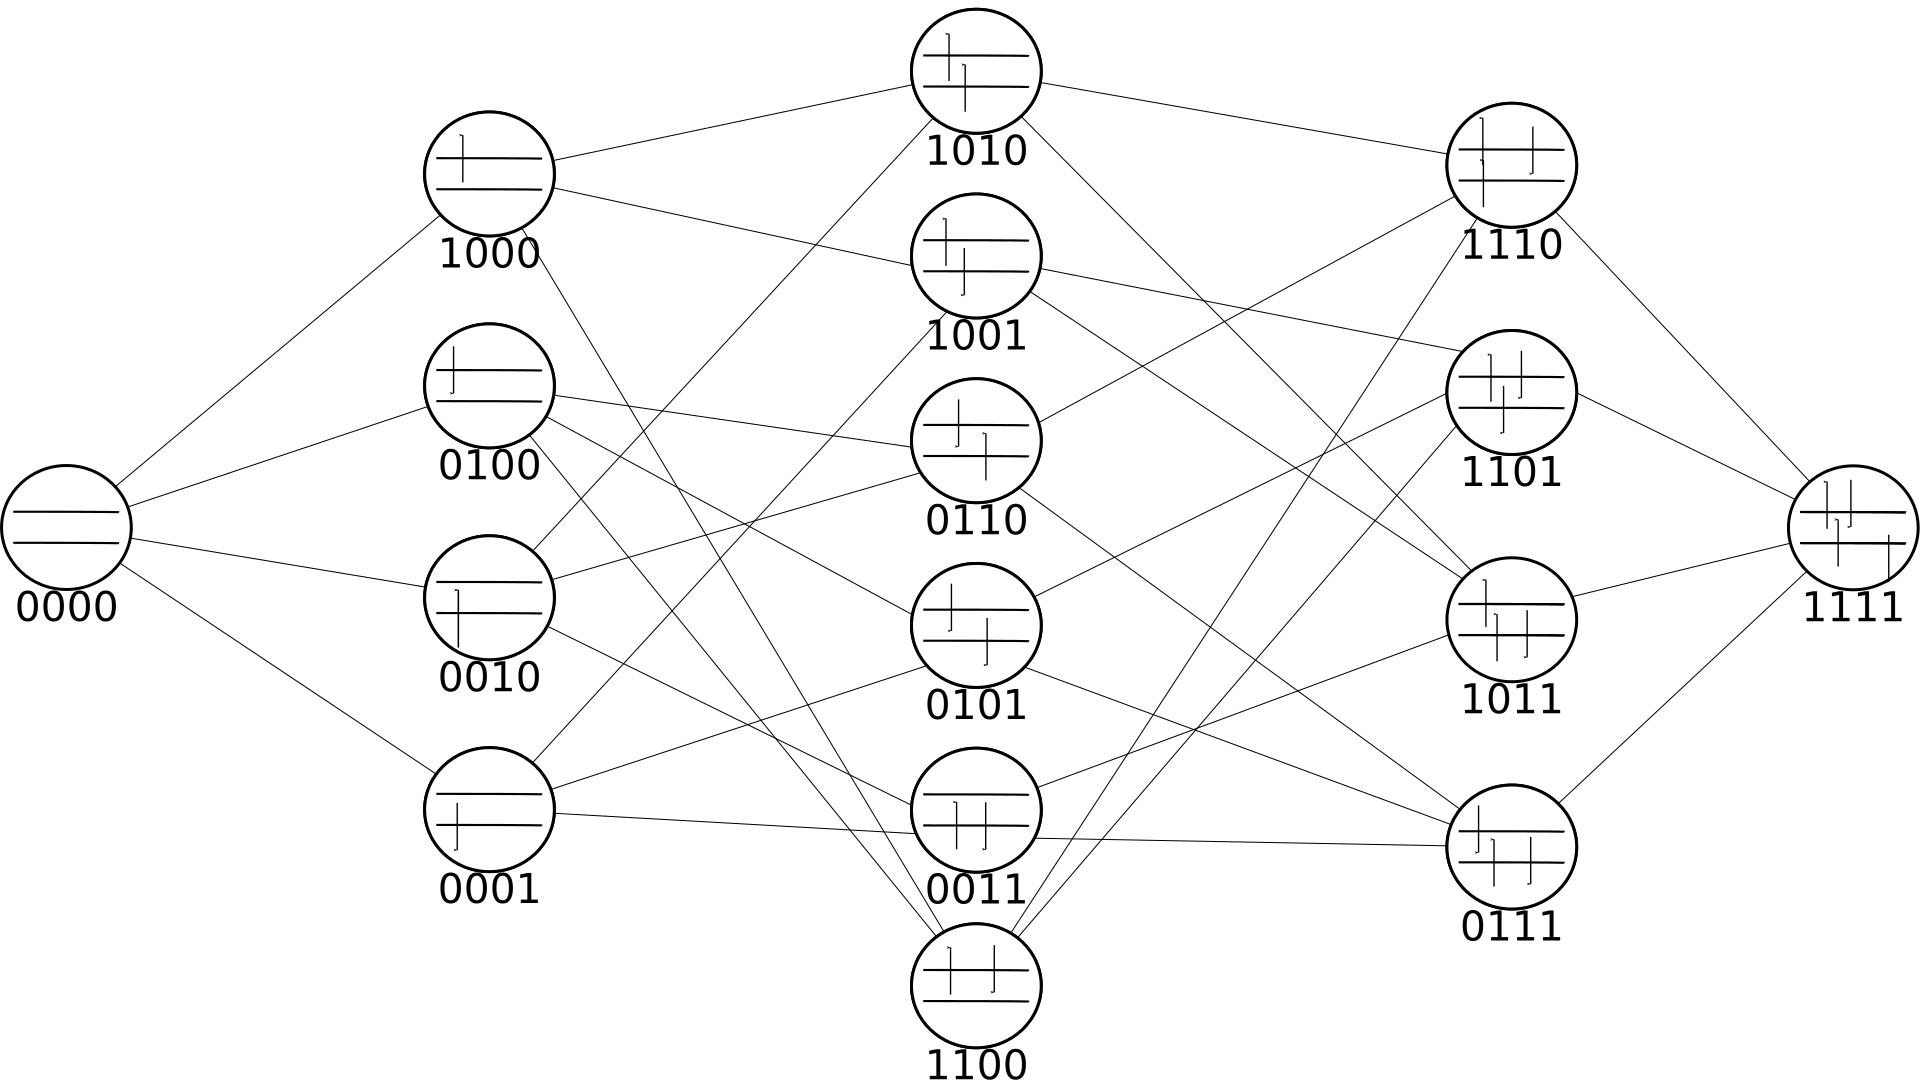
\includegraphics[scale=0.3]{level-graph.pdf}}
	\caption{Граф состояний двухуровневой системы}
	\label{fig:level-graph1}
\end{figure}

Таким образом можно сразу ввести эффективное, с точки зрения затрат вычислительных ресурсов, правило определения возможности перехода системы из одного зарядового состояния в другое: акт туннелирования возможен если побитовая запись номеров этих двух состояний отличается в одном и только в одном разряде. Для удобства дальнейшего повествования имеет смысл ввести логическую функцию $Graph(n, n')$, отвечающую правилу определения возможности перехода
\begin{equation}\label{rule}
Graph(n, n') =  \left\{
  \begin{array}{c}
    1\;\mbox{если переход $n \to n'$ возможен}\;,\\
    0\;\mbox{если переход $n \to n'$ невозможен}\;.
  \end{array}
  \right.
\end{equation}
$n$ и $n'$ здесь номера некоторых зарядовых состояний. 

\section{Система кинетических уравнений}
В данной работе для расчёта тока будет использоваться метод решения системы кинетических уравнений \cite{kinetic}. Изложим идею этого метода.

Введём в рассмотрение дискретную функцию $\sigma(n)$, определенную на множестве зарядовых состояний. Пускай в каждой точке она принимает значение, равное вероятности системы находится в зарядовом состоянии $n$. Отметим что для описанной двухуровневой системы данная функция будет определена в 16 точках. Вполне естественно требовать от значений данной функции выполнения условия нормировки:
\begin{equation}\label{norm}
\sum\limits_{i=0}^{15}\sigma(i) = 1
\end{equation}
Для состояний, переходы между которыми разрешены, справедливо управляющее уравнение("master equation"):
\begin{equation}\label{master}
\frac{d\sigma(n)}{dt} = \sum_{n \neq n'} \Gamma_{n,n'} \sigma(n') - \Gamma_{n',n} \sigma(n)
\end{equation}
Здесь $\Gamma_{n',n}$ есть темп туннелирования из состояния $n$ в состояние $n'$. Процесс с повышением номера зарядового состояния($n' > n$) эквивалентен туннелированию электрона на активный элемент. Следовательно, в таком случае:
\begin{equation}
\Gamma_{n',n} = \Gamma_{n',n}^{(L)} + \Gamma_{n',n}^{(R)}
\end{equation}
где $\Gamma_{n',n}^{(L)}$, $\Gamma_{n',n}^{(R)}$ — рассчитанные по формуле \ref{eq2} темпы туннелирования для левого и правого туннельного перехода соответственно. Для случая ($n' < n$) имеем обратную ситуацию:
\begin{equation}
\Gamma_{n',n} = \Gamma_{n',n}^{(L)} + \Gamma_{n',n}^{(R)}
\end{equation}
Электрон покидает зарядовый остров, а темпы туннелирования входящие в последнее соотношения рассчитываются по формуле \ref{eq4}.

Вернёмся к управляющем уравнению. Будем рассматривать только стационарный случай $(d\sigma(n)/{dt} = 0 , \forall n)$.  Приближение стационарности справедливо, если частоты, на которых будет работать устройство, меньше $1/\tau_0$, где $\tau_0$ — характерное время релаксации прибора. Левая часть уравнения \ref{master} зануляется. Для наглядности выпишем управляющее уравнение для зарядового состояния $n = 0$.
\begin{equation}
\Gamma_{0, 8} \sigma(8) + \Gamma_{0, 4} \sigma(4) + \Gamma_{0, 2} \sigma(2) +\Gamma_{0, 1} \sigma(1) - (\Gamma_{8, 0} + \Gamma_{4, 0} + \Gamma_{2, 0} + \Gamma_{1, 0})\sigma(0) = 0
\end{equation}
Количество подобных уравнений равно количеству зарядовых состояний. Таким образом мы получаем однородную систему линейных уравнений относительно коэффициентов $\sigma(n)$: 
\begin{equation}\label{kinetic_system}
\hat \Gamma \vec{\sigma} = \vec{\theta}
\end{equation}
Пусть $\gamma_{ij}$ — элемент матрицы $\hat \Gamma$. Тогда множители в уравнении \ref{kinetic_system} определены следующим образом:
\begin{equation}
\vec{\sigma} = \left(
\begin{array}{c}
  \sigma(0)\\
  \sigma(1)\\
 \vdots\\
  \sigma(14)\\
  \sigma(15)\\
  \end{array}
  \right),   \gamma_{ij}=
  \left\{
  \begin{array}{c}
    \Gamma_{j,i}\;\mbox{если}\;i \neq j \mbox{ и }\ Graph(n, n') = 1,\\
    \sum\limits_{Graph(i, k) = 1} -\Gamma_{i,k} \;\mbox{если}\;i = j, \\
    0 \mbox{ в любом другом случае }\\\
  \end{array}
  \right.
\end{equation}

Чтобы выделить однозначное решение, вспомним про условие нормировки \ref{norm} и заменим любую строку в системе на строку единиц. Данную систему можно решать стандартными численными методами  линейной алгебры. Стоит отметить, что матрица системы кинетических уравнений (\ref{kinetic_system}) разрежена.

\section{Расчёт транспортных характеристик}
После решения системы \ref{kinetic_system} задача о нахождении тока не представляет сложности. Теперь нам известны вероятности нахождения системы в каждом из зарядовых состояний. Будем считать, что если электрон движется по цепи в направлении от стока к истоку, он даёт положительный вклад в общую силу тока, а если наоборот, то отрицательный. Введём в рассмотрение две компоненты туннельного тока. Компонента $I^+$ будет равна суммарному туннельному току всех тех процессов, что идут с повышением номера зарядового состояния. Компонента $I^-$ ответственна за туннельный ток процессов с понижением этого числа. Выпишем в явном виде формулы для расчёта этих компонент
\begin{equation}\label{i_plus}
I^+ = \sum\limits_{
\begin{array}{c}
Graph(i,j) = 1 \\
 j > i \\
\end{array}
} \sigma(i)(\Gamma_{j,i}^{(R)} - \Gamma_{j,i}^{(L)})
\end{equation}
\begin{equation}\label{i_minus}
I^- = \sum\limits_{
\begin{array}{c}
Graph(i,j) = 1 \\
 j < i \\
\end{array}
} \sigma(i)(\Gamma_{j,i}^{(L)} - \Gamma_{j,i}^{(R)})
\end{equation}
Очевидно, что интересующая нас полная сила тока даётся соотношением:
\begin{equation}\label{i}
I = I^+ + I^-
\end{equation}

Теперь, когда мы умеем рассчитывать силу тока при фиксированном значении параметров, имеет смысл рассчитать её при вариации внешних параметров в некотором диапазоне. Таким образом можно получить следующие типы диаграмм:
\begin{description}

\item[\itshape (a)] Диаграммы зарядовой стабильности. Представляют собой зависимость модуля плотности тока $|I|$ от напряжения смещения $v_t = \varphi_d - \varphi_s$ и напряжения на затворе $v_g$
\item[\itshape (b), (c)] Вольт-амперные характеристики и сигнальные характеристики демонстрируют естественные для одноэлектронных устройств явления кулоновской блокады и ступеней.
\item[\itshape (d)] Зависимость среднего числа электронов на активном элементе $<n>$ от тех же $v_t$ и $v_g$
\end{description}

\section{Обсуждение результатов}

Раз мы для простоты начали рассматривать систему с двумя уровнями, то результаты для начала представим для неё
\thisfloatsetup{floatrowsep=mysep}
\begin{figure}[h!]
\begin{floatrow}
   \ffigbox{\caption{Диаграмма стабильности системы с 2 уровнями}\label{fig:current_2lvl}}
           {\includegraphics[scale = 0.6]{current 2lvl}}
   \ffigbox{\caption{Среднее число электронов для системы с 2 уровнями}\label{fig:n_2lvl}}
           {\includegraphics[scale = 0.6]{n 2lvl}}  
\end{floatrow}    
\end{figure}
\thisfloatsetup{floatrowsep=mysep}
\begin{figure}[h!]
\begin{floatrow}
   \ffigbox{\caption{ВАХ для системы с двумя уровнями}\label{fig:VAH_2lvl}}
           {\includegraphics[scale = 0.5]{VAH 2lvl}}
   \ffigbox{\caption{Сигнальная характеристика для системы с 2 уровнями}\label{fig:signal}}
           {\includegraphics[scale = 0.5]{signal 2lvl}}  
\end{floatrow}    
\end{figure}
Как можно заметить, использованные в данной работе методы позволяют строить любые необходимые диаграммы. Однако, модель с двумя уровнями всё же является некоторой абстракцией, поведение которой на реальных системах заметить невозможно. Поэтому вниманию читателя представляется диаграмма стабильности для системы с 8 уровнями.
\begin{figure}[h]
	\center{\includegraphics[scale=0.5]{2}}
	\caption{Диаграмма стабильности для системы с 8 уровнями}
	\label{fig:8lvl}
\end{figure}
Так же стоит обратить внимание на экспериментальные диаграммы 
полученные в работе \cite{SASET_EXP_OUR}, изображённые на рис.\ref{fig:exp1} и рис.\ref{fig:exp2}.
\thisfloatsetup{floatrowsep=mysep}
\begin{figure}[h!]
\begin{floatrow}
   \ffigbox{\caption{Модуль тока из эксперимента}\label{fig:exp1}}
           {\includegraphics[scale = 0.35]{SASET exp our}}
   \ffigbox{\caption{Проводимость из эксперимента}\label{fig:exp2}}
           {\includegraphics[scale = 0.35]{SASET exp our der}}  
\end{floatrow}    
\end{figure}
Стоит заметить, что асимптотическое поведение экспериментальной диаграммы с рис.\ref{fig:exp1} очень хорошо прослеживается на диаграмме, полученной с помощью моделирования на рис.\ref{fig:8lvl}. А наклонные прямые на экспериментальной диаграмме проводимости на рис.\ref{fig:exp2} можно проследить на рассчитанной  диаграмме на рис.\ref{fig:current_2lvl}.

\chapter*{Итоги}
\addcontentsline{toc}{chapter}{Итоги}
Программа, моделирующая работу одноатомного транзистора была написана на языке C++, без использования сторонних библиотек. Данное ПО является полностью оригинальным. Преобразование данных расчёта в изображения производилось с помощью языка Python и библиотек NumPy, Matplotlib.

В заключении следует отметить несколько моментов, требующих доработки. Во-первых, приближение для значения $\tau$ является очень грубым и предполагает, что электрод и атом разделяет прямоугольный потенциальный барьер, что разумеется не так см. рис.\ref{fig:barrier}. 
\begin{figure}[h!]
	\center{\includegraphics[scale=0.3]{барьер}}
	\caption{Распределение потенциала в реальной системе и модели}
	\label{fig:barrier}
\end{figure}

Во-вторых, на вычисление интегралов в уравнениях (\ref{eq2}) и (\ref{eq4}) приходится огромная часть времени выполнения программы. Осмысленным является создание массива табличных значений данного интеграла и хранение его в виде отдельного файла для мгновенного доступа программы к значению интеграла.

В-третьих, необходимо применение алгоритмов работы с разреженными матрицами для решения системы кинетических уравнений, т.к. размер данной матрицы экспоненциально растёт с увеличением количества свободных мест для электронов на атомных оболочках, а матрица системы остаётся заполненной преимущественно нулями.
\renewcommand\bibname{Cписок литературы}
\addcontentsline{toc}{chapter}{Cписок литературы}
\begin{thebibliography}{99}
	\bibitem{Fulton_Dolan} T. A. Fulton and G. J. Dolan. Phys. Rev. Lett., 59:109–112, Jul 1987.
	\bibitem{Amman}M. Amman, K. Mullen, and E. Ben-Jacob. Journal of Applied Physics, 65(1):339–346,
1989.
	\bibitem{Likharev}D.V. Averin and K.K. Likharev. Single electronics: A correlated transfer of single
electrons and cooper pairs in systems of small tunnel junctions. In B.L. ALTSHULER,
P.A. LEE, and R.A. WEBB, editors, Mesoscopic Phenomena in Solids, volume 30 of
Modern Problems in Condensed Matter Sciences, chapter 6, pages 173–271. Elsevier,
1991.
	\bibitem{Thermo} J. P. Pekola, J. K. Suoknuuti, J. P. Kauppinen, M. Weiss, P. v. d. Linden, and A. G. M.
Jansen. Coulomb blockade thermometry in the milli-kelvin temperature range in high
magnetic fields. Journal of Low Temperature Physics, 128(5):263–269, Sep 2002.
	\bibitem{memory} K. Nakazato, R. J. Blaikie, and H. Ahmed. Single-electron memory. Journal of Applied
Physics, 75(10):5123–5134, 1994.
	\bibitem{sensor} Knobel, R., Cleland, A. Nanometre-scale displacement sensing using a single electron transistor. Nature 424, 291–293 (2003).
	\bibitem{SASET_EXP_OUR} V. V. Shorokhov, D. E. Presnov, S. V. Amitonov, Yu. A. Pashkin, and V. A. Krupenin.Single-electron tunneling through an individual arsenic dopant in silicon
Nanoscale, 9:613–620, 2017.
	\bibitem{SMSET} Kubatkin, S., Danilov, A., Hjort, M. et al. Single-electron transistor of a single organic molecule with access to several redox states. Nature 425, 698–701 (2003).
	\bibitem{neuro} Bose, S., Lawrence, C., Liu, Z. et al. Evolution of a designless nanoparticle network into reconfigurable Boolean logic. Nature Nanotech 10, 1048–1052 (2015).
	\bibitem{Dobr} D. M. Dobrynin, V. V. Shorokhov, and V. A. Krupenin. Correlated parallel electron
transport in double- and triple-island single-electron transistors. Journal of Physics:
Conference Series, 1482:012027, mar 2020.
	\bibitem{SASET1} Park, J., Pasupathy, A. N., Goldsmith, J. I., Chang, C., Yaish, Y., Petta, J. R., … Ralph, D. C. (2002). Coulomb blockade and the Kondo effect in single-atom transistors. Nature, 417(6890), 722–725.
	\bibitem{Hubbard} Hubbard J. 1963Electron correlations in narrow energy bandsProc. R. Soc. Lond. A276238–257
	\bibitem{tJ} J. Spa lek, A. Lewicki, Z. Tarnawski, J. K. Furdyna, R. R. Ga l¸azka, Z.
Obuszko, Phys. Rev B 33, 3407 (1986)
    \bibitem{Masl} Maslova, N.S., Arseyev, P.I.  Mantsevich, V.N. Tunneling current and noise of entangled electrons in correlated double quantum dot. Sci Rep 11, 9336 (2021).
	\bibitem{patriot} Dagesyan, S.A., Shorokhov, V.V., Presnov, D.E., Soldatov, E.S., Trifonov, A.S., and Krupenin, V.A. Sequential reduction of the silicon single-electron transistor structure to atomic scale. Nanotechnology 28 (2017), 225304.
	\bibitem{Landau}Л.Д.Ландау, Е.М.Лифшиц Электродинамика сплошных сред М., Наука, 1982
	\bibitem{MMF} Свешников А.Г., Боголюбов А.Н., Кравцов В.В. Лекции по математической физике: Учеб. пособие. — М.: Издательство МГУ, 1993. — 352с.
	\bibitem{kinetic} Alexander N. Korotkov. Coulomb blockade and digital single-electron devices, 1996.
\end{thebibliography}

\end{document}
